\section{Unity 3D} % (fold)
\label{sec:unity_3d}

\subsection{O Unity }
\label{sub:o_unity}
	A unidade é um IDE de desenvolvimento de jogos com um potente mecanismo de renderização e totalmente integrado com um conjunto de ferramentas que permitem criação de conteúdos interativos em várias plataformas e em  3d ou 2d. Além disso é possível gerar builds para de 16 plataformas  como o linux , android ,windows e iOS com um alto nivel de qualidade pois é possível utilizar recursos prontos da Assert Store e de comunidades de compartilhamento de conhecimentos. 
	Para esse projeto foi escolhido o Unity i,pois  além dos benefícios citados acima com ele é possível que o desenvolvimento seja mais ágil, em menos tempo e com um custo menor e com uma qualidade razoável. 

\subsection{Workflow} % (fold)
\label{sub:workflow}
	Com o intuito de simplificar o processo de criação e produção de software, o Unity oferece um ambiente de trabalho com diversas ferramentas integradas para o desenvolvimento para a possibilitar a criação de mundos complexos com bloco de construção de cenas rapidamente escaláveis, implementar fluxos de controle utilizando linguagens altamente utilizadas no mercado como C\# e Java Script, com uma perfomace de tempo de compilação. Além disso durante o processo de criação é possível economizar tempo utilizando modelagens prontas, salas e forúm de bate papo para distribuição de conhecimentos e resolução de problemas e dúvidas.

\begin{figure}[h]
  \centering
  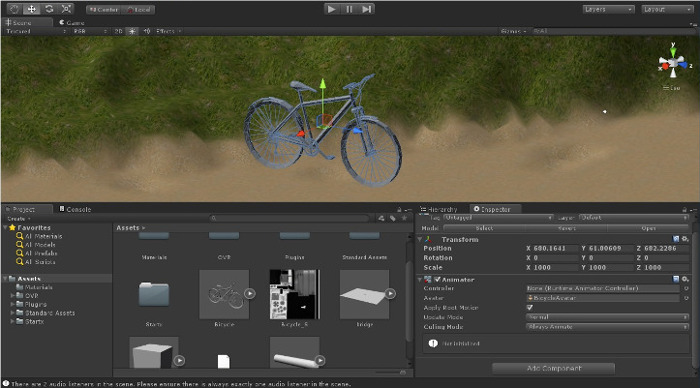
\includegraphics[width=0.8\textwidth]
      {figuras/bike.png}
  \caption{Edição de objeto no Unity}
  \label{coordenadas-rift}
\end{figure}

\subsection{Modelagem de Elementos} % (fold)
\label{sub:modelagem}
	Para a utilização de elementos no Unity é necessário a criação de objetos 3d, para isso pode ser utilizado qualquer um das IDE mais utilizadas do mercado tais como Maya , 3DMax, Blender ,Cinema4D, Modo, Lightwave, Cheetah3D, entre outros. A manipulação e ajustes de objetos em 3D está sendo realizada através da utilização da ferramenta Blender  que é uma plataforma livre de alto desempenho que permite além da modelagem para a criação de objetos 3D, contém ferramentas para animações, criação de jogos, construção de foto realismo, simulações de fluidos, edição de vídeos,entre outros.Depois de feito os ajustes nos modelos o Blender possui suporte para exportar objetos nos formatos de arquivo: 3DS,DXF,FBX,OBJ,LWO,SVG,STL entre outros.

\begin{figure}[h]
  \centering
  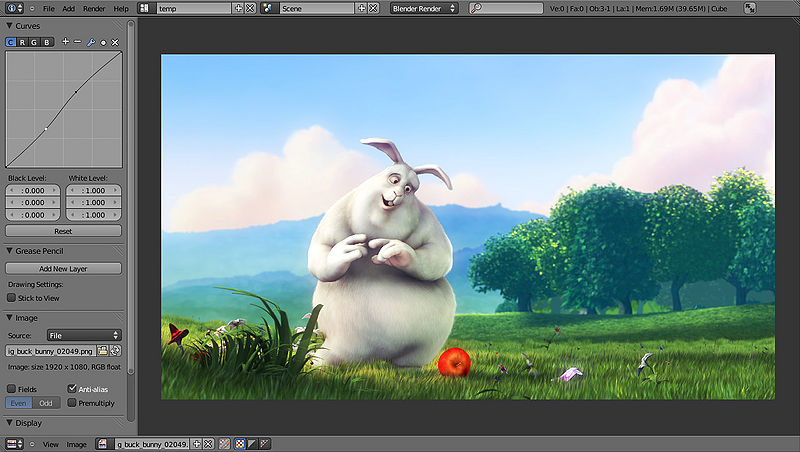
\includegraphics[width=0.8\textwidth]
      {figuras/blender.png}
  \caption{Renderização de \textit{Bick Buck Bunny} sendo feita no Blender}
  \label{coordenadas-rift}
\end{figure}

\subsection{SDK OculusVR}
\label{sub:sdk_ovr}
      Nos primeiros passos para a integração do Oculus Rift com o Unity foi necessário a utilização de uma SDK\footnote{ SDK encontrada em \url{https://developer.oculusvr.com/?action=dl&v=8 }} do próprio Oculus Rift, que atualmente possui as versões 0.2, 0.3 e 0.4, permite extrair dados do oculus e manipulos utilizando C++. No entanto como o Unity possui suporte para o plugin do Oculus Rift, que são scripts oriundos da SDK que ao invés de ser implementada em C++ é implementada em C\#, foi adotado o mesmo para auxiliar no controle do ambiente virtual no Unity.
     Com o plugin do Oculus Rift no Unity é possível controlar 2 cameras(que representa o campo visual do oculus em um usuário), e visualizar todo um ambiente em volta, utilizando os sensores da bicicleta e o Oculus Rift será possível controlar a bicicleta e movimentar a cabeça para aproveitar o ambiente virtual.

\subsection{Criação de Scripts}
\label{sub:criacao_de_scripts}
       A linguagem de programação utilizada nos scripts da SDK é o C\#, esta linguagem tem as caracteristicas de ser: orientada a objetos, dirigida a enventos, possui gerenciador de memória em tempo runtime( igual ao mente ao java o Garbage Collector é utilizado para liberar áreas de memória não utilizadas depois que uma classe é instanciada utilizando o operador new), e suporte a código legado.
       Esta linguagem possui tipos de dados como tipo de valor ou tipo de referência. Tipo de valor contém dados deste tipo e tipo de referência contém um inteiro apontando para uma area especifica da memória que irá conter os dados. Os tipos de valores normalmente representam dados simples como int e bool,  os tipos de referências são mais utilizados em strings e objetos. Os desenvolvedores podem contruir 3 tipos de dados de referências: classes , interfaces e delegados( tem a representação de um ponteiro de função em C, no entanto com a palavra chave delegados).As variaveis nesta linguagem podem ser do tipo Static(valor declarado fica disponivel para todos os objetos da classe que foi declarada), Instance(variável criada na memoria a cada vez que um  objeto é instanciado ) e Array (grupo de elementos do mesmo tipo de dados).
      Em C\# a unidade de programação é a Classe.Os objetos são instâncias(criações) destas classes , e suas funções são encapsuladas dentro dos limites  das classes e dos métodos.Em C\# as classes possui herança única , no entanto podem ser realizadas implementações de multiplas interfaces.Esta linguagem possui também um suporte a struct(Estrutura formada utilizando um conjunto de funções e variáveis), vinda do da linguagem C.O que é mais interessante nesta linguagem é a utilização de delegates ,que são referencias de métodos encapsulados com assinatura e tipo de retorno definido,onde é utilizada basicamente para invocar métodos indiretamente.
      Abaixo é ilustrado um exemplo de codigo em C\#, para a alteração do vetor direção da bicicleta e da modelagem 3D da bicicleta: 
 
\begin{lstlisting}
float current_position = 0;

public virtual void UpdatePlayerForwardDirTransform(){
	if ((DirXform != null) && (CameraController != null)) {
				//capturar botao D e rotacionar para a Direita
				if (Input.GetKey(KeyCode.D)) {
						current_position += 3f;
				}

				// capturar o botao A e rotacionar para a Esquerda
				if (Input.GetKey (KeyCode.A)) {
						current_position -= 3f;
				}

				//vetor identidade
				Quaternion i = Quaternion.identity;

				// rotataciona a bicicleta
				Quaternion d = Quaternion.Euler (new Vector3 (90, current_position, 0));
				Bicycle.rotation = i * d;

				//rotaciona o vetor direçao
				d = Quaternion.Euler (new Vector3 (0, current_position + 2f, 0));
				DirXform.rotation = i * d ;

				///escreve arquivo 
				write_position();
				write_rotation();
				write_altitude();
		}
}
\end{lstlisting}

